\documentclass{article}
%\usepackage[spanish,activeacute]{babel}
%\usepackage[english,activeacute]{babel}
%\usepackage[latin1]{inputenc}
\usepackage[utf8]{inputenc}
\usepackage[english]{babel}

\usepackage{amsmath,amsfonts,amssymb,amstext,amsthm,amscd}
\usepackage{hyperref}
\usepackage{latexsym}
\usepackage{graphicx}
%\usepackage{subfigure}
\usepackage{subfig}
%\linespread{1.6}
\usepackage{float}
\usepackage{dcolumn}% Align table columns on decimal point(esto lo saque del ejemplo de revtex4)
\usepackage{bm}% bold math(esto lo saque del ejemplo de revtex4)
\newcounter{itemR}
\usepackage{here} %recordar usar el comando[H] para las gráficas que es el comando here en lugar de [h!]
\usepackage{fancyhdr}
%\usepackage{sidecap}
%\usepackage[spanish,activeacute]{babel}
\usepackage{multirow}
\usepackage{multicol}
\usepackage{array}
\usepackage{enumitem}
\usepackage{listings}
%\usepackage{booktabs}% para hacer tablas profesionales con \toprule

% ------------------------------------------------------------------------------------------------------------------------------------------------------

\usepackage{fancyhdr}
\setlength{\headheight}{15.2pt}
\usepackage[paperwidth=8.5in, paperheight=11.0in, top=1.0in, bottom=1.0in, left=1.0in, right=1.0in]{geometry}
\lstnewenvironment{code}{\lstset{basicstyle=\ttfamily}}{}

\pagestyle{fancyplain}
\fancyhead[LE,RO]{Reporte análisis de algoritmos}
\fancyhead[CE,CO]{}
\fancyhead[RE,LO]{O23-LIS2012-1}
\fancyfoot[LE,RO]{\thepage}
\fancyfoot[CE,CO]{Matemáticas discretas, UDLAP}
\fancyfoot[RE,LO]{}

% ------------------------------------------------------------------------------------------------------------------------------------------------------
% ------------------------------------------------------------------------------------------------------------------------------------------------------
\begin{document}
\fancypagestyle{plain}{
   	\renewcommand{\headrulewidth}{1pt}
   	\renewcommand{\footrulewidth}{1pt}
}
\renewcommand{\footrulewidth}{1pt}
\renewcommand{\tablename}{Tabla}
\renewcommand{\figurename}{Figura}

% ------------------------------------------------------------------------------------------------------------------------------------------------------
% ------------------------------------------------------------------------------------------------------------------------------------------------------

\title{Análisis de algoritmos}
\author{\small{Erick Gonzalez Parada ID: 178145}\\
	   \small{Matemáticas discretas, Universidad de las Américas Puebla, Puebla, M\'exico}}
\date{\small{\today}}
\maketitle

% ------------------------------------------------------------------------------------------------------------------------------------------------------
% ------------------------------------------------------------------------------------------------------------------------------------------------------

\begin{abstract}
Análisis de Quick Select Lomuto.\\
\\
\\
{\it Keywords:}  búsqueda de posición, algoritmo   
\\
\\
\end{abstract}

% ------------------------------------------------------------------------------------------------------------------------------------------------------

\section{Introducción}\label{Introducción}                              	% -------------------- Introducción
El algoritmo \textit{Quick Select} de Lomuto es una variante de esta en donde\\
notablemente se utiliza \textit{Quick Sort}, sin embargo, el objetivo del \textit{Quick Select}\\
sera encontrar el k-ésimo de un array no necesariamente ordenado.\\
IMPORTANTE: Se asume que el arreglo tiene al menos k posiciones (base de index 0).  
\section{Explicación del algoritmo}\label{explicacion}				% -------------------- Metodología 
Nota: en pseudocódigo los comentarios son denotas con un '\%' y no pueden contener acentos,\\
las asignaciones son con el siguiente combo de símbolos ':=' y la comparación se hace con\\
un solo signo de igual '='.
\begin{code}
  funcion quick_select(arreglo, izquierda, derecha, k)
    % Si el rango solo contiene un elemento, regresar ese elemento
    si izquierda = derecha
        regresar arreglo[izquierda]
    % Dividir el arreglo en dos partes
    pIndex := particion(arreglo, izquierda, derecha)
    % Si el indice del pivote es igual a k, regresar el elemento en esa posicion
    si k = pIndex
        regresar arreglo[k]
    % Si k es menor que el indice del pivote, buscar en la parte izquierda del arreglo
    sino si k < pIndex
        regresar quick_select(arreglo, izquierda, pIndex - 1, k)
    % Si k es mayor que el indice del pivote, buscar en la parte derecha del arreglo
    sino
        regresar quick_select(arreglo, pIndex + 1, derecha, k)

funcion particion(arreglo, izquierda, derecha)
    % Seleccionar el ultimo elemento como pivote
    pivote := arreglo[derecha]
    % Inicializar el indice de particion con el valor de izquierda
    pIndex := izquierda
    % Recorrer el arreglo desde izquierda hasta derecha - 1
    para i desde izquierda hasta derecha - 1
        % Si un elemento es menor o igual al pivote, intercambiarlo con el elemento en pIndex y aumentar pIndex
        si arreglo[i] <= pivote
            intercambiar(arreglo[i], arreglo[pIndex])
            pIndex := pIndex + 1
    % Intercambiar el elemento en pIndex con el pivote y regresar pIndex
    intercambiar(arreglo[pIndex], arreglo[derecha])
    regresar pIndex
\end{code}

\section{Análisis del algoritmo}\label{AdA}
\subsection*{mejor caso}
Para el mejor caso solo necesitaríamos ejecutar un bloque del algoritmo,\\
el que se sale por que nuestro array es de tamaño 1, es decir, que tenga solo 1 elemento. 
\begin{figure}[H]
  \centering
  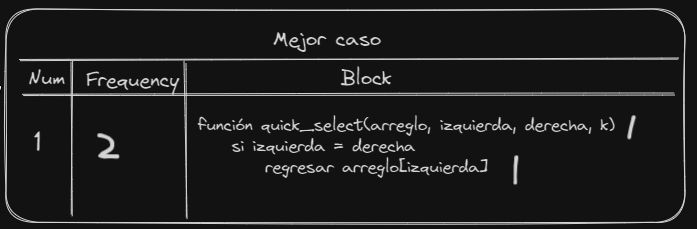
\includegraphics[scale=0.8]{../imgs/q2.png}
  \caption{Mejor caso}
  \label{Fig:1}
\end{figure}

  Función característica: 
  \begin{equation*}
    2 
  \end{equation*}
  Complejidad asintótica
  \begin{equation*}
    \Omega(2) = \Omega(k)
  \end{equation*}

  Donde k es la idea/concepto de una constante\\
  \\
  La gráfica de la complejidad asintótica es la siguiente: 
  \begin{figure}[H]
    \centering
    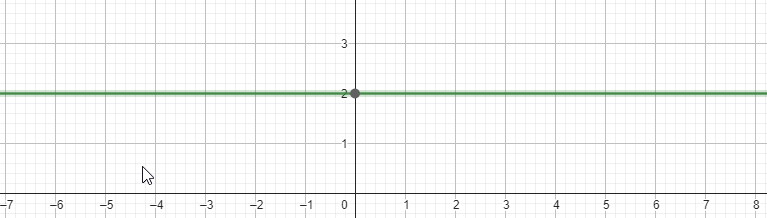
\includegraphics[scale=0.8]{../imgs/q4.png}
    \caption{Gráfica de caso de la fig \ref{Fig:1}}
    \label{Fig:2}
  \end{figure}

  Lo mejor del mundo en cuanto a velocidad (ver fig \ref{Fig:2}), una velocidad constante.
\subsection*{peor caso}
Para el peor caso tenemos:
\begin{figure}[H]
  \centering
  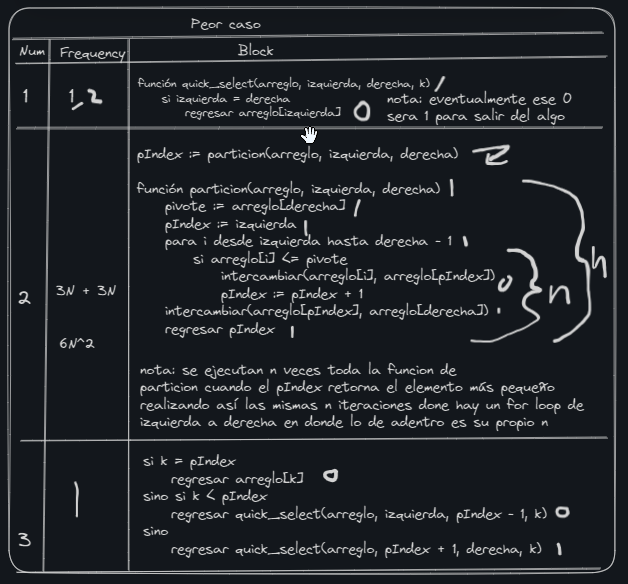
\includegraphics[scale=0.8]{../imgs/q3.png}
  \caption{Peor caso}
  \label{Fig:3}
\end{figure}

  Función característica: 
  \begin{equation*}
    2 + 6n^2 + 1 
  \end{equation*}
  Complejidad asintótica
  \begin{equation*}
    O(n^2) 
  \end{equation*}
  La gráfica de la complejidad asintótica es la siguiente: 
  \begin{figure}[H]
    \centering
    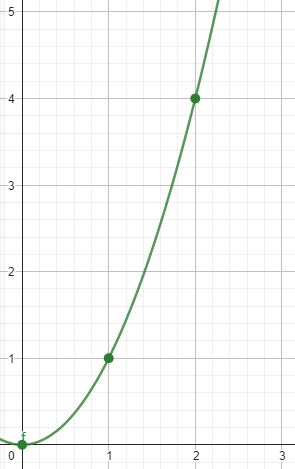
\includegraphics[scale=0.8]{../imgs/q5.png}
    \caption{Gráfica de caso de la fig \ref{Fig:3}}
    \label{Fig:4}
  \end{figure}
\section{Conclusiones}\label{Conclusiones}				% -------------------- Conclusiones
El algoritmo que evaluamos hoy \textit{quick search Lomuto} tiene la curiosidad de funcionar mejor\\
cuando el arreglo que se tiene esta de manera desordenada y funciona muy bien cuando tenemos muchos\\
datos ya que la complejidad asintótica promedio sera linealmente de \textit{n} sino en el pero caso\\
tenemos $\textit{n}^2$ como se puede observar en la fig \ref{Fig:4} y esto no lo queremos.
\end{document}	